\documentclass{beamer}
\usepackage[utf8]{inputenc}
\usepackage{textpos} 
\usepackage{graphicx} 
\usepackage{wrapfig}
\usepackage{tikz}
\usetikzlibrary{shapes.geometric,calc}

\usetheme{Boadilla}
\usecolortheme{default}



\title[Rapport Projet] 
{Rapport Projet sur la conception d'une application des gestion de projets informatiques}

\subtitle{Conception et élaboration d'un modèle suivant MERISE 2}

\author[HANFAOUI.K et KAFIF.I] 
{HANFAOUI Karim\inst{1} \and KAFIF. Imane\inst{2}}

\institute[EMSI] 
{
  \inst{1} EMSI, 3ème Année INFO G9\\
  \inst{2} EMSI, 3ème Année INFO G9
}

\date[DEC 2024] 
{EMSI Les Orangers, Décembre 2024}



\AtBeginSection[]
{
  \begin{frame}
    \frametitle{Table of Contents}
    \tableofcontents[currentsection]
  \end{frame}
}

\begin{document}



\begin{frame}
    \titlepage
    \begin{textblock*}{2cm}(9cm, -7.7cm) 
        \includegraphics[height=0.7cm]{logo} 
    \end{textblock*}
\end{frame}



\begin{frame}
\frametitle{Table of Contents}
\tableofcontents
\end{frame}

\begin{frame}
    \frametitle{List of Figures}
    \begin{itemize}
        \item \hyperlink{fig1}{Figure 1: Example Image}
        \item \hyperlink{fig2}{Figure 2: Another Example}
        \item \hyperlink{fig3}{Figure 3: Yet Another Example}
        \item \hyperlink{fig4}{Illustration des Événements dans le système}
        \item \hyperlink{fig5}{Illustration des Opérations}
        \item \hyperlink{fig6}{Illustration de la Synchronisation}
        \item \hyperlink{fig7}{Illustration des Résultats}
    \end{itemize}
\end{frame}


\section{Problématique}
\begin{frame}{C'est quoi notre Problématique}
    \begin{block}{Problématique}
        Comment concevoir et développer une application de gestion de projets informatiques capable de répondre efficacement aux besoins des équipes de développement en termes de suivi de l'avancement des projets, de gestion optimale des ressources, et de facilitation de la communication et de la collaboration, tout en s'adaptant aux contraintes organisationnelles et technologiques variées des entreprises ?
    \end{block}
\end{frame}

\section{Acronymes et Terminologie}
\begin{frame}{Acronymes et Terminologie}
    \textbf{MERISE} : Méthode d'Étude et de Réalisation Informatique pour les Systèmes d'Entreprise \\
    \textbf{MCD} : Modèle Conceptuel de Données \\
    \textbf{MLD} : Modèle Logique de Données \\
    \textbf{MCT} : Modèle Conceptuel de Traitement \\
    \textbf{MOT} : Modèle Organisationnel des Traitements \\
    \textbf{MCTA} : Modèle Conceptuel des Traitements Automatisés \\
    \textbf{MOTA} : Modèle Organisationnel des Traitements Automatisés \\
    \textbf{UML} : Unified Modeling Language (Langage de Modélisation Unifié) \\
    \textbf{USE CASE} : Cas d’Utilisation, outils de l'UML \\
    \textbf{Réseau de Petri} : Modèle mathématique pour la modélisation et l’analyse des processus concurrents \\
\end{frame}


\section{Résumé du cours}
\begin{frame}{La Conception d’un Système d’Information (SI)}
    \begin{itemize}
        \item \textbf{Nécessité stratégique} : Répondre aux besoins actuels et évoluer avec l’organisation.
        \item \textbf{Objectifs} :
        \begin{itemize}
            \item Optimiser les opérations courantes.
            \item Préparer aux défis futurs.
        \end{itemize}
        \item \textbf{Importance} : Garantir des systèmes efficaces et adaptés aux entreprises.
    \end{itemize}
\end{frame}

\begin{frame}{Critères de Qualité d’un Logiciel}
    \begin{itemize}
        \item \textbf{Utilité} : Répondre précisément aux besoins.
        \item \textbf{Utilisabilité} : Facilité d'apprentissage et d'interaction.
        \item \textbf{Fiabilité} : Fonctionnement sans défaillance.
        \item \textbf{Interopérabilité} : Interaction avec d'autres systèmes.
        \item \textbf{Performance} : Rapidité et efficacité en gestion des ressources.
        \item \textbf{Portabilité} : Adaptabilité à différents environnements.
        \item \textbf{Réutilisabilité} : Réutilisation des composants.
        \item \textbf{Facilité de maintenance} : Correction et mise à jour aisées.
    \end{itemize}
\end{frame}

\begin{frame}{Cycle de Vie du Logiciel : Étapes}
    \begin{enumerate}
        \item \textbf{Analyse des besoins et des risques} : Étude de faisabilité.
        \item \textbf{Spécification} : Cahier des charges fonctionnelles et techniques.
        \item \textbf{Conception} : Définition de l'architecture et des interfaces.
        \item \textbf{Codage} : Traduction des spécifications en code source.
        \item \textbf{Tests} : Vérification et validation.
        \item \textbf{Livraison} : Déploiement et formation des utilisateurs.
        \item \textbf{Maintenance} : Correction, amélioration et adaptation.
    \end{enumerate}
\end{frame}

\begin{frame}{Modèles de Cycle de Vie}
    \begin{itemize}
        \item \textbf{Modèle en cascade} : Processus séquentiel, validation étape par étape.
        \item \textbf{Modèle itératif et incrémental} : Développement par cycles avec ajout progressif de fonctionnalités.
        \item \textbf{Méthodes agiles} :
        \begin{itemize}
            \item Exemples : Scrum, Kanban.
            \item Itérations courtes avec adaptation rapide aux changements.
        \end{itemize}
    \end{itemize}
\end{frame}

\begin{frame}{Documents Produits dans le Cycle de Vie}
    \begin{itemize}
        \item \textbf{Cahier des charges} : Définition des besoins fonctionnels et techniques.
        \item \textbf{Calendrier du projet} : Planification des étapes et livrables.
        \item \textbf{Plan de test} : Objectifs et stratégies de validation.
        \item \textbf{Plan d'assurance qualité} : Standards pour garantir la qualité.
        \item \textbf{Manuel utilisateur} : Guide pratique pour les utilisateurs.
        \item \textbf{Code source} : Instructions codées représentant le logiciel.
        \item \textbf{Rapport des tests} : Résultats des tests effectués.
        \item \textbf{Rapport des défauts} : Liste des anomalies et corrections.
    \end{itemize}
\end{frame}

\begin{frame}{Modélisation : Définition et Rôle}
    \begin{itemize}
        \item \textbf{Définition} : Représentation abstraite de la réalité pour concevoir des logiciels structurés.
        \item \textbf{Rôles du modèle} :
        \begin{itemize}
            \item Document d’échange entre clients et développeurs.
            \item Outil de conception.
            \item Référence pour le développement et la maintenance.
        \end{itemize}
    \end{itemize}
\end{frame}

\begin{frame}{Méthodes de Modélisation}
    \begin{itemize}
        \item \textbf{MERISE} :
        \begin{itemize}
            \item MCD : Modèle Conceptuel de Données.
            \item MCT : Modèle Conceptuel des Traitements.
            \item MLD : Modèle Logique des Données.
        \end{itemize}
        \item \textbf{UML (Unified Modeling Language)} :
        \begin{itemize}
            \item Diagrammes : Cas d'utilisation, classes, séquences.
        \end{itemize}
        \item \textbf{Modélisation orientée objets} :
        \begin{itemize}
            \item Décomposition en objets autonomes et interactifs.
        \end{itemize}
    \end{itemize}
\end{frame}

\begin{frame}
    \frametitle{Figure 1: Example Image}
    \label{fig1}
    \begin{figure}
        \includegraphics[width=0.8\textwidth]{logo}
        \caption{This is an example image.}
    \end{figure}
\end{frame}

\begin{frame}
    \frametitle{Figure 2: Another Example}
    \label{fig2}
    \begin{figure}
        \includegraphics[width=0.8\textwidth]{logo}
        \caption{This is another example image.}
    \end{figure}
\end{frame}

\begin{frame}
    \frametitle{Figure 3: Yet Another Example}
    \label{fig3}
    \begin{figure}
        \includegraphics[width=0.8\textwidth]{logo}
        \caption{Yet another example image.}
    \end{figure}
\end{frame}


\section{Comparaison entre Merise 1 et Merise 2}

\begin{frame}{Qu'est-ce que MERISE 1 ?}
\begin{itemize}
    \item MERISE 1 est une méthodologie française d’analyse et de conception des systèmes d’information.
    \item Développée dans les années 1970, elle est utilisée pour modéliser et réaliser des bases de données et des applications.
\end{itemize}
\end{frame}

\begin{frame}{Principes fondamentaux de MERISE 1}
\begin{enumerate}
    \item \textbf{Séparation des niveaux de modélisation :}
    \begin{itemize}
        \item Modèle conceptuel (niveau conceptuel)
        \item Modèle logique (niveau organisationnel)
        \item Modèle physique (niveau technique)
    \end{itemize}
    \item \textbf{Cycle de vie du système d’information :}
    \begin{itemize}
        \item Étude préalable, étude détaillée, réalisation, exploitation et maintenance.
    \end{itemize}
    \item \textbf{Focus sur les données :}
    \begin{itemize}
        \item Modèle Conceptuel des Données (MCD)
        \item Modèle Logique des Données (MLD)
        \item Modèle Physique des Données (MPD)
    \end{itemize}
\end{enumerate}
\end{frame}

\begin{frame}{Caractéristiques de MERISE 1}
\begin{itemize}
    \item Approche systématique, adaptée aux projets bien définis et peu évolutifs.
    \item Centré sur les bases de données relationnelles.
    \item Modélisation utilisant des diagrammes (MCD, MCT, DFD).
\end{itemize}
\end{frame}

\begin{frame}{Limites de MERISE 1}
\begin{itemize}
    \item Peu adapté aux systèmes modernes (orientés objet, dynamiques).
    \item Approche rigide, difficilement compatible avec des méthodologies agiles.
\end{itemize}
\end{frame}
\begin{frame}{Qu'est-ce que MERISE 2 ?}
\begin{itemize}
    \item MERISE 2 est une évolution de MERISE 1, adaptée aux systèmes d’information modernes.
    \item Introduite pour intégrer les technologies récentes comme les bases orientées objet et les architectures distribuées.
    \item Offre une flexibilité accrue grâce à des concepts enrichis et à une approche plus évolutive.
\end{itemize}
\end{frame}

\begin{frame}{Principes fondamentaux de MERISE 2}
\begin{enumerate}
    \item \textbf{Extension des niveaux de modélisation :}
    \begin{itemize}
        \item Modèle conceptuel enrichi pour intégrer les cycles de vie des données.
        \item Modèle logique et physique adaptés aux bases orientées objet.
    \end{itemize}
    \item \textbf{Prise en compte des objets :}
    \begin{itemize}
        \item Gestion des classes, objets, et relations dynamiques.
        \item Insistance sur les interactions entre objets et leurs états.
    \end{itemize}
    \item \textbf{Cycle de développement souple :}
    \begin{itemize}
        \item Permet des itérations fréquentes pour s’adapter aux évolutions du projet.
    \end{itemize}
\end{enumerate}
\end{frame}

\begin{frame}{Caractéristiques de MERISE 2}
\begin{itemize}
    \item Intègre les paradigmes orientés objet pour une modélisation plus moderne.
    \item Convient aux bases relationnelles et orientées objet.
    \item Approche plus souple, adaptée aux systèmes évolutifs et complexes.
    \item Utilisation des mêmes outils de modélisation (MCD, MLD, MPD) avec des extensions.
\end{itemize}
\end{frame}

\begin{frame}{Limites de MERISE 2}
\begin{itemize}
    \item Méthodologie complexe, nécessitant une expertise pour sa mise en œuvre.
    \item Moins populaire que les méthodologies modernes comme UML ou les approches agiles.
    \item Peut être lourde pour des projets de petite envergure.
\end{itemize}
\end{frame}

\begin{frame}{Comparaison entre MERISE 1 et MERISE 2}
\begin{table}[]
\resizebox{\textwidth}{!}{%
\begin{tabular}{|l|l|l|}
\hline
\textbf{Critères}             & \textbf{MERISE 1}                                                   & \textbf{MERISE 2}                                                    \\ \hline
\textbf{Orientation}          & Centrée sur les flux de données et traitements                     & Intègre une approche orientée objet                                  \\ \hline
\textbf{Technologie ciblée}   & Bases de données relationnelles classiques                         & Bases relationnelles et orientées objet                              \\ \hline
\textbf{Modélisation}         & Modèles conceptuels, logiques et physiques classiques (MCD, MLD)   & Modèles enrichis (cycles de vie des objets et interactions dynamiques) \\ \hline
\textbf{Flexibilité}          & Rigide, séquentielle                                               & Souple, itérative                                                    \\ \hline
\textbf{Adaptabilité}         & Convient aux projets bien définis et peu évolutifs                 & Convient aux projets évolutifs et modernes                           \\ \hline
\textbf{Complexité}           & Plus simple                                                       & Plus complexe, mais mieux adapté aux systèmes modernes               \\ \hline
\textbf{Popularité actuelle}  & Rarement utilisé aujourd'hui                                       & Moins populaire que UML et les approches agiles                      \\ \hline
\end{tabular}%
}
\end{table}
\end{frame}

\end{frame}

\section{Présentation du modèle conceptuel du traitement analytique}

\begin{frame}{MCTA C'est quoi ?}
    \textbf{En modélisation informatique, notamment dans la méthode Merise}, le MCTA fait référence au 
    \textbf{Modèle Conceptuel des Traitements et des Activités}. C'est une étape clé pour décrire comment les processus et les traitements fonctionnent dans un système d'information.
    
    \vspace{1em}
    \textbf{Rôle du MCTA dans Merise :}
    \begin{itemize}
        \item Le MCTA intervient après le Modèle Conceptuel des Données (MCD).
        \item Il se concentre sur les activités et traitements nécessaires pour manipuler les données.
        \item L'objectif est de décrire les flux, interactions et règles de gestion sans s'intéresser à l'aspect technique.
    \end{itemize}
    
    \vspace{1em}
    \textbf{Diagrammes associés :}
    \begin{itemize}
        \item \textbf{Diagrammes d'activités} pour montrer les enchaînements.
        \item \textbf{Modèles conceptuels de flux (MCF)} pour représenter les flux de données entre traitements.
    \end{itemize}

\end{frame}

\begin{frame}{idk if we should keep this '-'}

    
    \textbf{Différence avec le Modèle Logique des Traitements (MLT) :}
    \begin{itemize}
        \item \textbf{MCTA} : Vision conceptuelle, indépendante de l'implémentation technique.
        \item \textbf{MLT} : Vision plus proche de l'implémentation informatique (scripts, programmes).
    \end{itemize}
    
\end{frame}

\begin{frame}{Événements dans le MCTA}
    \textbf{Événements :} Eux qui déclenchent les activités /ou traitements dans le système.
    \begin{itemize}
        \item Correspondent aux stimuli externes ou internes qui démarrent un processus.
        \item Représenté par un ovale avec le nom et/ou description à l'intérieur 
        \item \textbf{Exemples :}
        \begin{itemize}
            \item Un client passe une commande.
            \item Un paiement est reçu.
            \item Une alerte est générée en cas de problème.
        \end{itemize}
    \end{itemize}
    \vspace{1em}
    \label{fig4}
    \begin{figure}
        \centering
        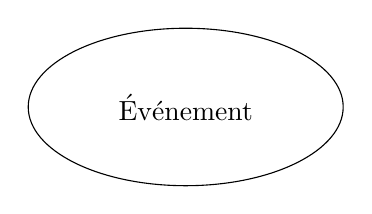
\begin{tikzpicture}
    \draw[fill=none, draw=black] (0,0) ellipse (2cm and 1cm); % Dessiner un ovale avec des dimensions réduites et couleur invisible
    \node at (0, 0) {Événement}; % Placer le texte "Événement" au centre de l'ovale
\end{tikzpicture}
        \caption{Illustration des Événements dans le système}
    \end{figure}
\end{frame}

\begin{frame}{Opérations dans le MCTA}
    \textbf{Opérations :} Actions spécifiques réalisées par le système pour transformer les données.
    \begin{itemize}
        \item Correspondent aux unités élémentaires d'un traitement.
        \item \textbf{Exemples :}
        \begin{itemize}
            \item Calculer le total d'une commande.
            \item Mettre à jour le stock.
            \item Valider une transaction.
        \end{itemize}
    \end{itemize}
    \vspace{1em}
    \label{fig5}
    \begin{figure}
        \centering
        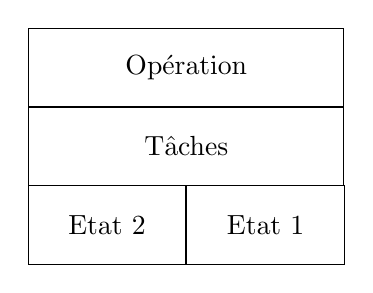
\begin{tikzpicture}
  \node (op) [rectangle, draw, minimum width=4cm, minimum height=1cm] {Opération};
  \node (taches) [rectangle, draw, minimum width=4cm, minimum height=1cm, below of=op] {Tâches};
  \node (etat1) [rectangle, draw, minimum width=2cm, minimum height=1cm, below of=taches, anchor=west] {Etat 1};
  \node (etat2) [rectangle, draw, minimum width=2cm, minimum height=1cm, below of=taches, anchor=east] {Etat 2};
\end{tikzpicture}
        \caption{Illustration des Opérations}
    \end{figure}
\end{frame}


\begin{frame}{Synchronisation dans le MCTA}
    \textbf{Synchronisation :} Régule l'ordre d'exécution des traitements.
    \begin{itemize}
        \item Assure que les traitements se déroulent dans un ordre cohérent.
        \item \textbf{Exemples :}
        \begin{itemize}
            \item Un paiement doit être validé avant l'expédition d'une commande.
            \item Plusieurs traitements doivent s'exécuter simultanément.
            \item Une activité attend la fin d'autres activités avant de se déclencher.
        \end{itemize}
    \end{itemize}
    \vspace{1em}
    \label{fig6}
    \begin{figure}
        \centering
        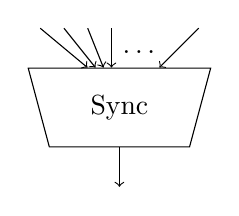
\begin{tikzpicture}
  \node (trap) [trapezium, draw, minimum width=2cm, minimum height=1cm, trapezium left angle=-75, trapezium right angle=-75, node contents={Sync}] {};
  \draw[<-] (trap.south) ++(0,-0.5) -- ++(0,0.5);  
  %\draw[<-] (trap.north west) -- ++(0,0.5);
  \draw[<-] ($(trap.north west)!0.1!(trap.north east)$) -- ++(-0.6,0.5);
  \draw[<-] ($(trap.north west)!0.2!(trap.north east)$) -- ++(-0.4,0.5);
  \draw[<-] ($(trap.north west)!0.3!(trap.north east)$) -- ++(-0.2,0.5);
  \draw[<-] ($(trap.north west)!0.4!(trap.north east)$) -- ++(0,0.5);
  \node at ($(trap.north west)!0.5!(trap.north) + (0.5,0.2)$) {$\dots$}; 
  \draw[<-] (trap.north east) -- ++(0.5,0.5); 
\end{tikzpicture}
        \caption{Illustration de la Synchronisation}
    \end{figure}
\end{frame}
\begin{frame}
\frametitle{Synchronisation dans le MCTA}

\begin{alertblock}{Remarque :}
\footnotesize Les règles représentant la synchronisation peuvent être composées et on obtient aisément la forme générale :
\[P = \sum_{i=1}^{n} \left( \prod_{j=1}^{m_i} L_{i,j} \right)\]
où: 
\begin{itemize}
    \item $P$ est le résultat de sortie.
    \item $L_{i,j}$ est un prédicat logique (un évènement arbitraire).
    \item $\sum_{i=1}^{n} m_i$ est le nombre total d'événements.
\end{itemize}
\end{alertblock}
\end{frame}

\begin{frame}{Un exemple de Sync:}

\begin{examples}
\ex a ET b \\
\footnotesize Pour obtenir cette expression à partir de la forme générale on fixe les paramètres suivants :

* $n = 1$ (une seule clause)
* $m_1 = 2$ (deux littéraux dans la clause)
* $L_{1,1} = a$
* $L_{1,2} = b$

En substituant ces valeurs dans la forme générale, on obtient :

\[\sum_{i=1}^{1} \left( \prod_{j=1}^{2} L_{i,j} \right) = \prod_{j=1}^{2} L_{1,j} = L_{1,1} \land L_{1,2} = a \land b\]
\end{examples}
    
\end{frame}

\begin{frame}{Un autre exemple de Sync composé}
\begin{examples}
\ex a OU b ET c \\
\footnotesize Pour obtenir cette expression à partir de la forme générale 
\[\sum_{i=1}^{n} \left( \prod_{j=1}^{m_i} L_{i,j} \right),\] 
on fixe les paramètres suivants :

* $n = 2$ (deux clauses)
* $m_1 = 1$ (un littéral dans la première clause)
* $m_2 = 2$ (deux littéraux dans la deuxième clause)
* $L_{1,1} = a$
* $L_{2,1} = b$
* $L_{2,2} = c$

En substituant ces valeurs dans la forme générale, on obtient :

\begin{align*}
\sum_{i=1}^{2} \left( \prod_{j=1}^{m_i} L_{i,j} \right) &= \left( \prod_{j=1}^{1} L_{1,j} \right) \lor \left( \prod_{j=1}^{2} L_{2,j} \right) \\
&= L_{1,1} \lor (L_{2,1} \land L_{2,2}) \\
&= a \lor (b \land c) \\
&= a \lor (b \land c)
\end{align*}
\end{examples}
\end{frame}


\begin{frame}{Résultats dans le MCTA}
    \textbf{Résultats :} Les sorties des activités ou traitements.
    \begin{itemize}
        \item Correspondent aux effets observables ou données produites après une opération.
        \item Représenté par un ovale avec le nom et/ou description à l'intérieur
        \item \textbf{Exemples :}
        \begin{itemize}
            \item Une facture générée pour un client.
            \item Un email de confirmation envoyé.
            \item Une mise à jour dans une base de données.
        \end{itemize}
    \end{itemize}
    \vspace{1em}
    \begin{figure}
        \centering
        \label{fig7}
        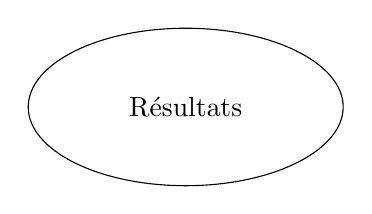
\begin{tikzpicture}
    \draw[fill=none, draw=black] (0,0) ellipse (2cm and 1cm); % Dessiner un ovale avec des dimensions réduites et couleur invisible
    \node at (0, 0) {Résultats}; % Placer le texte "Événement" au centre de l'ovale
\end{tikzpicture}
        \caption{Illustration des Résultats}
    \end{figure}
\end{frame}

\begin{frame}{Représentation Final du MCTA}
i swear its 1:07AM i cant do this anymore i gtg to sleep
\end{frame}

\section{Conception du projet selon les règles de Merise 2}
\begin{frame}{Conception selon Merise 2}
    Explication des règles et de leur application au projet.
\end{frame}

\section{Bibliographies et Références}
\begin{frame}{Bibliographies}
\begin{thebibliography}{9}

\bibitem{bts_doc}
BTS CGO 2A P10 -\textit{ Organisation du Système d’Informations Fiche MCT, MCTA, MOT et MOTA.} Editions d'Organisation. 
\href{https://example.com/merise}{[Lien]} 

\bibitem{merise_miseaniveau}
Pr. S.EL MOUMNI -\textit{ Conception des systèmes d’information.} Cours mise à niveau. 
\alert{[Lien non disponible]}

\end{thebibliography}
\end{frame}

\begin{frame}
\frametitle{Sample frame title}

In this slide, some important text will be
\alert{highlighted} because it's important.
Please, don't abuse it.

\begin{block}{Remark}
Sample text
\end{block}

\begin{alertblock}{Important theorem}
Sample text in red box
\end{alertblock}

\begin{examples}
Sample text in green box. The title of the block is ``Examples".
\end{examples}
\end{frame}



\begin{frame}
\frametitle{Two-column slide}

\begin{columns}

\column{0.5\textwidth}
This is a text in first column.
$$E=mc^2$$
\begin{itemize}
\item First item
\item Second item
\end{itemize}

\column{0.5\textwidth}
This text will be in the second column
and on a second thought, this is a nice-looking
layout in some cases.
\end{columns}
\end{frame}


\end{document}
